\documentclass{article}
\usepackage{graphicx}
\usepackage{xcolor}
\usepackage{subcaption}
\usepackage[margin=1.0in]{geometry}
\usepackage{float}
\usepackage{ulem}
\usepackage{amsmath}
\usepackage{mathtools}
\usepackage{wrapfig}

\begin{document}
\section{Introduction}

\section{Methods}
\subsection{Density Matrix Downfolding (DMD)}
The DMD procedure allows us to develop low-energy effective theories for physical systems in a systematic manner beginning with the \textit{ab-initio} Hamiltonian:
\begin{equation}
\hat{H}_\text{ab} = -\frac{1}{2} \sum_{i} \nabla_i^2 - \sum_{i,I}\frac{Z}{|r_i - R_I|} + \sum_{i<j}\frac{1}{|r_i - r_j|}
\label{eq:Hab}
\end{equation}
where $i$ indicates electrons and $I$ nuclei, and the unit of energy is Hartree (Ha).
In this paper we will be working under the Born-Oppenheimer approximation and core electrons will be treated using pseudo-potentials.
The procedure defines a method for downfolding the \textit{ab-initio} energy functional and Hilbert space onto an effective energy functional defined on a low-energy subspace of the Hilbert space 
\begin{equation}
(E_\text{ab}, \mathcal{H}) \xrightarrow{\text{DMD}} (E_\text{eff}, \mathcal{LE} \subset \mathcal{H}), \text{ s.t. }
\forall |\Psi\rangle \in \mathcal{LE}, \ E_\text{eff}[\Psi] - E_\text{ab}[\Psi] = \epsilon[\Psi] + E_0.
\label{eq:DMD}
\end{equation} 
The energy functionals can be written as expectations over Hamiltonian operators $E_\text{ab} = \langle \Psi | \hat{H}_\text{ab} |\Psi \rangle$, $E_\text{eff} = \langle \Psi | \hat{H}_\text{eff} |\Psi \rangle$, $\epsilon$ represents the error in our effective theory, and $E_0$ is a constant energy shift.
Broadly the DMD method consists of four steps which will be discussed in detail later: 
A) Defining the space of low-energy excitations which $E_\text{eff}$ should be able to describe accurately.
B) Sampling, at minimum, a set of states in $\mathcal{H}$ which probe the chosen low-energy excitations in a statistically independent manner. The selected states need not be eigenstates. 
C) Constructing a set of candidate models which are linear in reduced density matrix (RDM) descriptors with variable coefficients $\{c\}$
\begin{equation}
E_\text{eff} = \sum_k c_k \langle \Psi | \hat{d}_k |\Psi \rangle + E_0.
\label{eq:Eeff}
\end{equation}
Here $\hat{d}_k$ are Hermitian operators typically composed of 1- or 2-RDM elements. 
Examples of possible $\hat{d}_k$ are number operators $\hat{n}_i$ and exchange operators $\vec{S}_i \cdot \vec{S}_j$.
Additionally, a single particle basis must be built to express RDM elements on and should be chosen such that variations among states in $\mathcal{LE}$ are mostly described by variations in the projection of these states onto the basis.
D) Using the samples to fit the coefficients $\{c\}$ by linear regression such that $E_\text{eff}$ satisfies the conditions in \eqref{eq:DMD} with the smallest error $\epsilon$ possible. 
The fitting procedure is typically an ordinary linear regression, however, one may use a custom cost function in the regression as well. 
In order to conduct the linear regression for a functional like \eqref{eq:Eeff}, one needs to calculate for each state sampled from $\mathcal{LE}$ the expectation values of $\hat{H}_\text{ab}$ and every descriptor $\{\hat{d}_k\}$ used in the regression.
In principle, if conducted with no approximations, the DMD method is rigorously guaranteed to obtain exact results, namely $\epsilon[\Psi] = 0$.

\subsection{Fixed-node diffusion Monte Carlo (FN-DMC)}
When downfolding $\hat{H}_\text{ab}$ we will use FN-DMC to access states in $\mathcal{LE}$ and accurately calculate their \textit{ab-initio} energies and RDM elements.
Diffusion Monte Carlo (DMC) is a quantum Monte Carlo method which projects out the ground state of a Hamiltonian given some initial trial wave function.
Consider a trial wave function $|\Psi_T\rangle$ and the Hamiltonian $\hat{H}_\text{ab}$ with ground state $|\Phi_0\rangle$. We apply the projector $e^{-\tau \hat{H}_\text{ab}}$ as $\tau \rightarrow \infty$ to $|\Psi_T \rangle$
\begin{equation}
\lim_{\tau \rightarrow \infty} e^{-\tau \hat{H}_\text{ab}} |\Psi_T\rangle 
\equiv \lim_{\tau \rightarrow \infty} |\Psi_\text{DMC}(\tau)\rangle \propto \langle \Phi_0|\Psi_T\rangle |\Phi_0\rangle,
\end{equation}
projecting out the ground state as long as the trial wave function we choose is not orthogonal to the ground state. 
The stochastic implementation involves moving samples from the trial function $\Psi_T(R)$ using the Green function $G(R, R^\prime, \tau) = \langle R | e^{-\tau(\hat{H}_\text{ab} - E_T)} | R^\prime \rangle$. Since $H_\text{ab} = T + V$, kinetic and potential energy terms, the Green function is approximated by a Trotter expansion $G(R, R^\prime, \tau) = \langle R | e^{-\tau(\hat{H} - E_T)} | R^\prime \rangle \sim \Big[e^{-d\tau(V(R) + V(R^\prime))/2} \langle R| e^{-d\tau(\hat{T} - E_T)}|R^\prime \rangle + O(d\tau^2) \Big]^N $ where $d\tau = \tau/N$.
This expansion can be interpreted as an interative procedure where samples are moved N times with a small timestep $d\tau$ until convergence.
The constant $E_T$ is a trial energy used to control the normalization of $\Psi_\text{DMC}(\tau, R)$ and is updated at each move.
This implementation, however, suffers from a fermion sign problem. 
We deal with this sign problem through a fixed-node approximation, where the nodal surface of $\Psi_\text{DMC}(\tau, R)$ is forced to match that of the initial trial wave function for all $\tau$.
This approximation makes FN-DMC variational, and will only return the exact ground state of $\hat{H}_\text{ab}$ if the nodal surfaces of $|\Psi_T\rangle$ and $|\Phi_0\rangle$ are identical.
We make use of this variational principle to access low-energy states within $\mathcal{H}$ by choosing trial wave functions with nodes that differ from the nodes of $|\Phi_0 \rangle$.
To calculate the expectation value of an operator $\hat{A}$ in FN-DMC we will use a mixed estimator $\langle \Psi_{DMC}(\tau) |\hat{A} | \Psi_T \rangle/\langle \Psi_\text{DMC}(\tau) | \Psi_T \rangle$ which allows us to use the importance sampled distribution $f = \Psi_\text{DMC}(\tau)\Psi_T$ for our Monte Carlo estimates.
Details for calculating reduced density matrix elements in FN-DMC can be found in Wagner.

\subsection{Defining $\mathcal{LE}$ for CuO molecule}
We construct our $\mathcal{LE}$ based on recent anion photoelectron spectroscopy (APES) measurements of the low-lying excited states of the nuetral CuO molecule. 
The lowest energy excitations measured, which lie below 2eV, involve primarily the O 2p$_z$, 2p$_\pi$ and Cu 4s orbitals, which are fully-filled, half-filled and empty in the ground state respectively.
Beginning at 2.2 eV are excitations which remove a single electron from the fully filled Cu 3d shell and add them to either the O 2p$_\pi$ or Cu 4s orbitals.
Seeing that the lowest energy excitations of the CuO molecule involve removing at most one electron from the Cu 3d shell, we define our low-energy space as
\begin{equation}
\mathcal{LE} = \text{Span(}\{ |\Psi \rangle | \langle \Psi | \hat{n}_{3d} | \Psi \rangle \ge 9,\ \hat{H}_\text{ab}|\Psi\rangle = E |\Psi\rangle \}\text{)}.
\label{eq:LE}
\end{equation}
Our particular focus will be on describing most accurately the properties and energies of eigenstates up to $\sim$2eV, as measurements on higher energy states observe a nearly continuous block of states which include vibrational modes.

\subsection{Sampling $\mathcal{LE}$}
Our sample space was generated by using multi-Slater-Jastrow trial wavefunctions in FN-DMC. 
In principle we could probe every low-energy excitation in $\mathcal{LE}$ in a statistically independent manner by just sampling the eigenstates within $\mathcal{LE}$ and including various non-eigenstates within $\mathcal{LE}$ as well to ensure robust statistics.
In practice we do not have access to these eigenstates and approximate methods are required to sample the low-energy space. 
Consider a trial wavefunction of the form $e^{J_i} |\text{D}_i\rangle$, where $e^{J_i}$ is a three-body Jastrow factor and $|\text{D}_i\rangle$ is a determinant of some single particle orbitals.
If the nodes of $|\text{D}_i\rangle$ are similar to the nodes of an eigenstate $|\Phi_i\rangle \in \mathcal{LE}$, then the properties and energy calculated from FN-DMC using this trial wavefunction will approximate those of the eigenstate, with the degree of approximation depending on the quality of the trial function nodal structure.
If we were able to find for each $|\Phi_i \rangle \in \mathcal{LE}$ such a $|\text{D}_i\rangle$ then we can approximate any state in $\mathcal{LE}$ as
\begin{equation}
|\Psi\rangle = \sum_i c_i |\Phi_i\rangle \sim \sum_i c_i \lim_{\tau \rightarrow \infty} e^{-\tau \hat{H}_\text{ab}} (e^{J_i} |D_i\rangle) \xrightarrow{J_i = J} \lim_{\tau \rightarrow \infty} e^{-\tau \hat{H}_\text{ab}} (e^{J}\sum_{i} c_i|\text{D}_i\rangle).
\label{eq:sampling}
\end{equation}
The last equality is valid if $\forall i\  J_i = J$, allowing us to map $|\Psi \rangle \in \mathcal{LE}$ to the end result of an FN-DMC calculation using a multi-Slater-Jastrow trial wavefunction. We use symmetry-targeted unrestricted Kohn-Sham (UKS) to generate our determinants $|\text{D}_i\rangle$ using a B3LYP functional, which has been shown to accurately reproduce ground state nodal properties of transition-metal oxide molecules, a Trail-Needs pseudopotential, and the VTZ Trail-Needs basis using the package PySCF.
The symmetry-targeted UKS method allows us to fix the total spin projection S$_z$ and the total number of electrons in a particular irreducible representation (irrep) of the symmetry group under use, $\text{A},\ \text{E}_\text{1x},\ \text{E}_\text{2y}$ etc.
This method allows us to access almost every excitation in $\mathcal{LE}$, however, there are some cases of two or more low-energy states within $\mathcal{LE}$ which have identical S$_z$ and number of electrons per irrep.
An example of this dilemma would be the ground state and the state with an excitation from Cu 3d$_{xz} \rightarrow $  O 2p$_x$.
In these few cases the higher energy excited $|\text{D}_i\rangle$ is inaccessible and the corresponding $|\Phi_i\rangle$ is excluded from the sum in \eqref{eq:sampling}, restricting our sample space to a subspace of $\mathcal{LE}$.
Methods like constrained DFT also failed to converge the inaccessible $|\text{D}_i\rangle$.
We will discuss the consequences of this restriction later on.
A single three-body Jastrow factor $J$ was used for every $|\text{D}_i\rangle$ and was optimized on the lowest energy UKS state using a linear energy optimization method.
The FN-DMC calculations were conducted with T-moves, to make the calculation variational while using pseudopotentials, with a timestep of $\tau = 0.01$.
The coefficients $\{c_j\}$ for our sample states were chosen via a shell-sampling method. 
We begin by fixing the coefficient $c_0 = \sqrt{w}$ where $w \in \{1.0, 0.8, ..., 0.2\}$. 
For each choice of $w$ we sample n = 5 states by randomly selecting the unassigned coefficients from a uniform distribution such that $\sum_i c_i^2 = 1$. 
This procedure generates shells of samples at decreasing distance from the eigenstate $|\Phi_0\rangle$. 
We can then loop over all $i$ to generate shells near each eigenstate.
This sampling scheme tends to be sparse where the density of states of $\hat{H}_\text{ab}$ is low and therefore extra samples are generated in regions of sparse sample density \textit{post-hoc}. 

\subsection{Constructing candidate models}
Parameterizing our effective model requires constructing a basis on which to calculate our \textit{ab-initio} 1-/2-RDM elements and selecting a set of descriptors from which we would like to build our model.
As discussed, the lowest energy excitations in the CuO molecule are between the Cu 3d, 4s and O 2p orbitals, meaning that our basis needs to span these orbitals. 
We constructed two such bases: a localized intrinsic atomic orbital (IAO) basis and a molecular orbital (MO) basis.
The IAO basis was built on all Cu 3d, 4s and O 2p molecular orbitals from the $|\text{D}_i\rangle$ used to construct our sample states.
The MO basis consists of the Cu 3d, 4s and O 2p molecular orbitals from the lowest energy restricted open-shell Kohn-Sham (ROKS) solution with $x \leftrightarrow y$ spatial symmetry, a O 2p$_z \rightarrow$ O 2p$_\pi$ excitation.
As these two bases are used to describe the same space, they are related by an orthogonal transformation which will allow us to map between them if necessary.
This choice for the MO basis ensures that our basis elements are spin-independent and respect the spatial symmetries of the molecule.
In order to describe the low-energy degrees of freedom in the CuO molecule our model will require occupation energies and hybridizations between the Cu 3d, 4s and O 2p atomic orbitals.
A sparser representation can be found using a MO basis, since occupation operators in the MO basis contain information on both occupation and hybridization in an atomic basis. 
The lack of doubly occupied Cu 4s states in the low-energy spectrum of CuO indicate the necessity of a Hubbard U term on the Cu 4s.
This is corroborated by the fact that the FN-DMC energy of the lowest-lying sampled state with a doubly occupied Cu 4s orbital is 7 eV above the lowest energy sampled state.
Further, we include a Hund's coupling between the Cu 4s and Cu 3d orbitals in our model based on the existence of a similar Hund's coupling 
for the copper atom.
These two interaction terms are best represented in the IAO basis as they are intuitively interactions between localized orbitals.
In addition to these important parameters, we will consider models which contain any number of hybridizations between the MOs to account for orbital relaxation between excited states in the CuO molecule.
In total our space of canditate models is then 
\begin{equation}
\begin{split}
\{\bar{n}_{4s}, \bar{n}_{p_\pi}, \bar{n}_{p_z}, \hat{n}_{4s\uparrow} \hat{n}_{4s\downarrow},\sum_{i \in \{xy, xz, ...\}}\vec{S}_{4s}\cdot \vec{S}_{d_i}\} \ + \\
\text{P}(\bar{c}_{d_\pi}^\dagger \bar{c}_{p_\pi} + h.c.,\ \bar{c}_{d_z^2}^\dagger \bar{c}_{p_z} + h.c.,\ \bar{c}_{4s}^\dagger \bar{c}_{p_z} + h.c.,\ \bar{c}_{d_z^2}^\dagger \bar{c}_{4s} + h.c.)
\end{split}
\label{eq:models}
\end{equation}
where P denotes the power set and operators are defined on the IAO basis unless denoted by a bar, in which case the operator is built on the MO basis. The coefficients for each term above will be denoted $\bar{\epsilon}_{4s},\ \bar{\epsilon}_{p_\pi},\ \bar{\epsilon}_{p_z},\ U_s,\ J_{sd},\ \bar{t}_\pi,\ \bar{t}_{dz},\ \bar{t}_{sz},\ \bar{t}_{ds}$. The operator $\bar{n}_{3d}$ is not included in any models as it is linearly dependent on all other occupation energies through the relationship $\bar{n}_{3d} + \bar{n}_{p_z} + \bar{n}_{p_\pi} + \bar{n}_{4s} = N_\text{elec} = \text{15}$. The symbol $\pi$ denotes a contraction over $x, y$ for p orbitals and $xz,\ yz$ for d orbitals. The symbol $\delta$, introduced later, denotes a contraction over $xy,\ x^2-y^2$ for d orbitals.

\pagebreak
\subsection{Fitting candidate models}
After fitting each of the potential models in \eqref{eq:models} using ordinary linear regression (OLS) and solving the resultant models using exact diagonalization, we find a set of models which describe the energy functional on our sample set accurately but whose eigenstates and spectra differ as a consequence of intruder states below an energy of 2eV. 
The sixteen different models all regress with R$^2 >$ 0.95 on our sample data, however some models are more robust than others. 
Models which have coefficients that are zero within 95\% confidence intervals, computed through bootstrap estimates, are removed from consideration.
We then take the left over models, rotate every operator and coefficient into the IAO basis through an appropriate orthogonal transformation, and exactly diagonalize the models.
Any models which have an average errorbar in eigenvalues, also estimated by bootstrapping, greater than 0.25 eV are ignored.
Each of the remaining six models describe our sample set accurately, have robust non-zero coefficients, and have small error bars in eigenvalues.
However, the eigenstates below 2eV differ greatly between these models as illustrated in Figure \ref{fig:InitED}.

\begin{figure}[H]
\centering
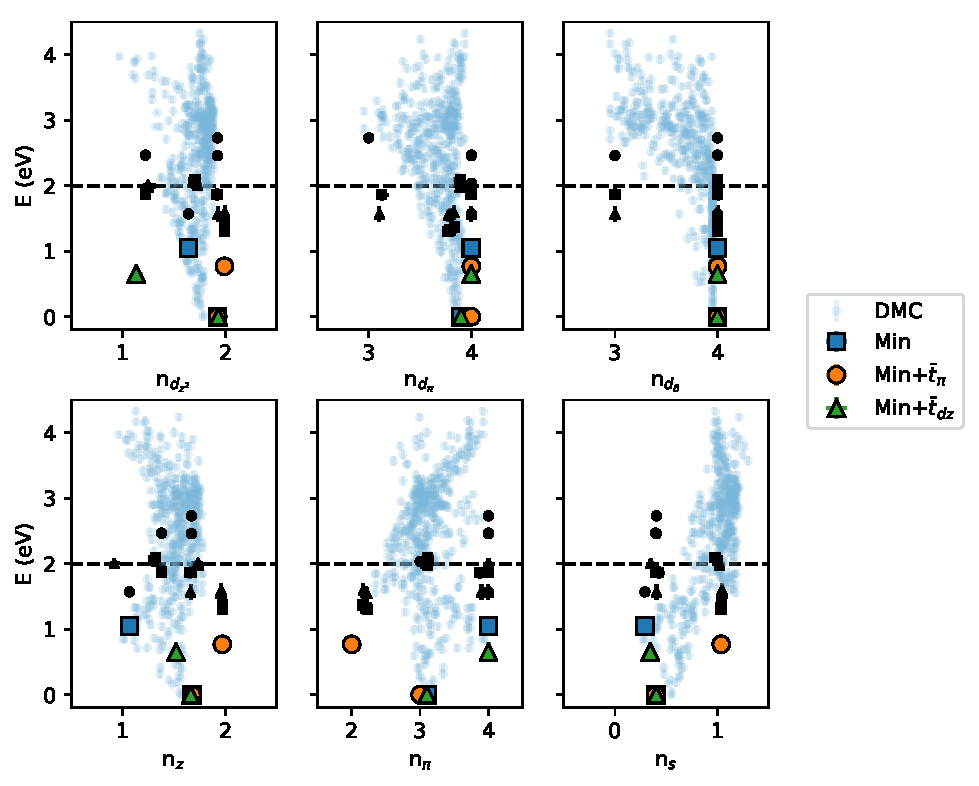
\includegraphics[width=0.7\linewidth]{../qwalk/old/ub3lyp_s1_/analysis/figs/init_ed.pdf}
\caption{Results of exact diagonalization showing the energies and properties of the first twenty eigenstates for three candidate models. The ground state and first excited state are colored and have enlarged markers for clarity.}
\label{fig:InitED}
\end{figure}

All three models have a first excited state around 1eV, but only in the minimal model does this state fall near the sample set used for the fitting, and is the only model in which this state corresponds to the correct excitation O 2$p_z \rightarrow $ O 2p$_\pi$ as seen in experiment.
In contrast, the first excited state for the other two models are visibly distant from our sample set and do not correspond to the experimental first excited state.
The large distance of these eigenstates from our sample set indicates that their predicted eigenvalues may suffer from large extrapolation errors, and as such we will call them \textit{intruder} states.
In Figure \ref{fig:Intruder} we present all eigenstates among the six potential models which we classify as intruders.
While using a Mahalanobis distance is a typical strategy for outlier (intruder) detection, it is only useful for distributions which are approximately normal.
Our sample space does not resemble a (multivariate) normal distribution in any way, so we instead look at the average distance of the five nearest neighbor samples to an eigenstate.
If the average distance is larger than 0.9, which in this case happens to divide eigenstates into intruders above and not below cleanly, it is classified as an intruder state.
In the situation that multiple models share an intruder state, only the intruder state with the farthest average distance is included.

\begin{figure}[H]
\centering
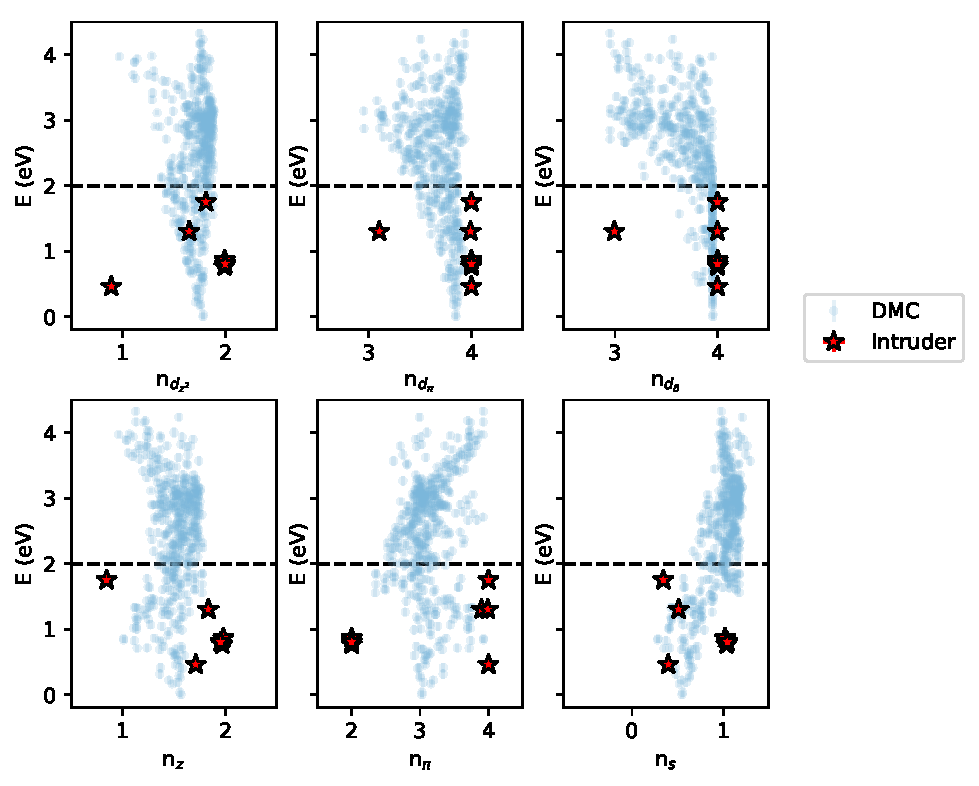
\includegraphics[width=0.7\linewidth]{../qwalk/old/ub3lyp_s1_/analysis/figs/intruder.pdf}
\caption{Collection of unique intruder states from our six potential models selected using a k-nearest neighbor approach with k = 5.}
\label{fig:Intruder}
\end{figure}

Given that our intruder states correspond to states within $\mathcal{LE}$ but outside our sample set, they must live within the span of the eigenstates which were excluded in our sampling scheme as described before.
This is evidenced by the fact that two of the intruder states correspond explicitly to excitations we could not access: Cu 3d$_{z^2} \rightarrow $ O 2p$_\pi$ and  Cu 3d$_\pi \rightarrow $ O 2p$_\pi$.
In fact, these are the only two singly excited states which we could not access with our sampling scheme.
While inaccessible, we can approximate these states by single rigid MO excitations above the UKS ground state, which results in states with a FN-DMC energy above 4eV.
Including a generous 2eV reduction in FN-DMC energy due to orbital relaxation, we estimate that these two states should lie at least 2eV in energy. 
Since all the other inaccessible eigenstates are double or higher order excitations, our very approximate exploration of the inaccessible parts of $\mathcal{LE}$ leaves us with a reasonable prior: intruder states should lie above 2eV in energy in our effective theories.
We can enforce this prior by adding a term to our ordinary linear regression cost function
\begin{equation}
\text{Cost} = \sum_{i} (E_\text{eff}[\Psi_i] - E_\text{ab}[\Psi_i])^2 + \lambda \sum_{p}\text{QHL}(2 - E_\text{eff}[\Psi_p]),\ \text{QHL}(x) = \Theta(x)x^2
\label{eq:cost}
\end{equation}
where $\lambda>0$ is a parameter which can be varied, QHL is a quadratic hinge loss, $\Theta$ is the Heaviside step function, the index $i$ is over our sampled states and $p$ over the selected intruder states.
Increasing the value of $\lambda$ leads to a stronger penalty for models which do not satisfy our prior.

\pagebreak
\section{Discussion}


\section{Conclusion}

\end{document}